\documentclass{article}

\newcommand{\authorname}{Austin Jetrin Maddison}
\newcommand{\course}{Discrete Simulation}
\newcommand{\courseid}{ICMA393}
\newcommand{\docname}{HW2}
\newcommand{\titletext}{\course: \docname}

%\usepackage{fontspec}	
\usepackage[no-math]{fontspec}	
\setmainfont{HelveticaNowText}
\newfontface\hh{HelveticaNowText-ExtraBold}
\newfontface\lt{HelveticaNowText-Light}      
\newfontface\xx{HelveticaNowText-ExtraLight} 
\newfontface\mm{HelveticaNowText Medium}

\newfontfamily{\displayfont}{HelveticaNowDisplay}
\newfontface\dslt{HelveticaNowDisplay-Light}
\newfontface\dsmm{HelveticaNowDisplay-Medium}
\newfontface\dsbd{HelveticaNowDisplay-Bold}

\newfontfamily{\microfont}{HelveticaNowMicro}
\newfontface\mclt{HelveticaNowMicro-Light}
\newfontface\mcmm{HelveticaNowMicro-Medium}
\newfontface\mcbd{HelveticaNowMicro-Bold}

\setmonofont{SFMono}

\usepackage[lining]{FiraSans}
\usepackage[fakebold]{firamath-otf}
\usepackage{unicode-math}
\setmathfont{FiraMath}
\renewcommand*\oldstylenums[1]{{\firaoldstyle #1}}


\usepackage{microtype}   % Improves text appearance with microtypography
\usepackage{amsmath}     % For better math support
\usepackage{graphicx}    % For including graphics
\usepackage{lipsum}      % For placeholder text
\usepackage{enumitem}
\usepackage{xcolor}
\usepackage{svg}
\usepackage{svg-extract}
\usepackage{caption}
\usepackage{float}
\usepackage{multicol}


\usepackage[a4paper, margin=0.8in, columnsep=20pt]{geometry}

\captionsetup{font=small}
\definecolor{gray}{rgb}{0.55, 0.55, 0.55}
\setlength{\columnsep}{20pt}  % Space between columns

% Headers and Footers
\usepackage{fancyhdr}
\pagestyle{fancy}
\fancyhf{}

% First Page
\fancypagestyle{plain}{
\fancyfoot[R]{\small \thepage} 
\fancyfoot[L]{} 
\fancyhead[L]{}
\fancyhead[R]{}
}

% Custom header
\fancyfoot[L]{\scriptsize \MakeUppercase{ \microfont \courseid~\course}}
\fancyhead[L]{\scriptsize \MakeUppercase{ \microfont \docname}}
\renewcommand{\headrulewidth}{0pt}

% Custom footer
%\fancyfoot[L]{\small Title, Date}
\fancyfoot[R]{\small \thepage}

% Line spacing
\usepackage{setspace}
\setstretch{1.15}  % Slightly more space between lines

%\setlength{\mathindent}{0pt} % This removes the indentation for equations

% Section formatting
\usepackage{titlesec}
\titleformat{\section}[block]{\large\dsbd}{\thesection.}{1em}{}
\titleformat{\subsection}[block]{\normalsize \mm}{\thesubsection.}{1em}{}

% Bibliography style
\usepackage[numbers,sort&compress]{natbib} % For numbered citations

% Hyperlinks
\usepackage{hyperref}
\hypersetup{
    colorlinks=false,
    linkcolor=blue,
    citecolor=blue,
    urlcolor=blue,
    pdftitle={Research Paper Title},
    pdfauthor={Author's Name},
}

\usepackage{listings}
\lstset{
  language=Python,                     % Use Python language syntax
  basicstyle=\ttfamily\footnotesize,           % Use modern monospace font for code
  keywordstyle=\bfseries\color{black},   % Bold and blue keywords
  stringstyle=\color{black},              % Strings in red
  commentstyle=\color{gray},            % Comments in gray
  showstringspaces=false,               % Don't show spaces in strings
  breaklines=true,                      % Break long lines
  tabsize=4,                            % Set tab size to 4 spaces
}


\begin{document}
\fontsize{9.5}{11.5}\selectfont % Set font size to 12pt with a baseline of 14pt

% Title 
\title{
  \raggedright
  \Large \displayfont \strong{\courseid~\titletext} \\[5pt]  % Adjust spacing if needed
%  \raggedleft
  \small Mahidol University International College \\
  \small \authorname \\ 
  \small \today
}
\date{} 

%
%\twocolumn[{
%	\vspace*{-1cm}
%	\maketitle
%	\vspace*{-0.5cm}
%}]

\maketitle
%\raggedbottom
\section{Archimedes Method of N-Gon}

a) 



\textbf{Calculate $\mathbf{p_3}$}

\begin{multicols}{2}

\begin{figure}[H]
	\centering
	
\includegraphics[width=1\linewidth]{../drawings/p1_1}
%	\caption{}
%	\label{fig:path1}
\end{figure}

\columnbreak

\begin{align*}
	p_{3}&=2d+2d+2d\\ 
	&=6d\\
	&=6\cdot\frac{\sqrt{3}}{2}\\ 
	&=3\sqrt{3}
\end{align*}

\end{multicols}

\textbf{Calculate $\mathbf{P_3}$}	

\begin{multicols}{2}
	
\begin{figure}[H]
	\centering
	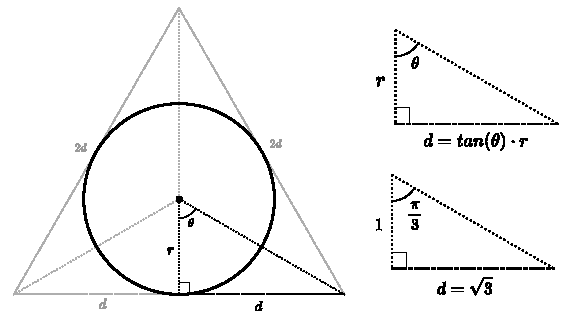
\includegraphics[width=1\linewidth]{../drawings/p1_2}
	%	\caption{}
	%	\label{fig:path2}
\end{figure}

\columnbreak

\begin{align*}
	P_{3}&=2d+2d+2d\\ 
	&=6d\\
	&=6\cdot\sqrt{3}\\ 
	&=6\sqrt{3}
\end{align*}
	
\end{multicols}

\noindent
b)
\begin{multicols}{2}
\begin{lstlisting}
P_6 , p_6  pi approx = 3.14614428  
pi                   = 3.14159265  
# matching digits 	 = 3

P_12, p_12 pi approx = 3.14187328  
pi                   = 3.14159265  
# matching digits 	 = 4

P_24, p_24 pi approx = 3.14161018  
pi                   = 3.14159265  
# matching digits 	 = 4

P_48, p_48 pi approx = 3.14159375  
pi                   = 3.14159265  
# matching digits 	 = 6

P_96, p_96 pi approx = 3.14159272  
pi                   = 3.14159265  
# matching digits 	 = 7

P_192, p_192 pi approx = 3.14159266  
pi                     = 3.14159265  
# matching digits 	   = 9

\end{lstlisting}

\end{multicols}




\pagebreak


\section{Approximate $\mathbf{\sqrt{2}}$}

a)  Summed all the n-terms of the taylor expansion of $\sqrt{2}$.
\\
\begin{lstlisting}
def f(n=150):
	x = 2
	sum = 0
	an = 1
	bn = 1/2
	
	for i in range(n):
		term = (an * (x - 1) ** bn) * (x - 1) ** i / math.factorial(i)
		sum += term
		
		an *= bn
		bn -= 1
	
	return sum
\end{lstlisting}
\vspace{10pt}
\noindent
$f()=1.4142909169379279$
\\
\\


\noindent
b) Approximate $\sqrt{2}$ by uniformly sampling uniform random numbers $x$ and counting whether $x^2$.
\\
\begin{multicols}{2}
\begin{lstlisting}
def f(n = 1000000, x=2):
	xs = np.random.ranf(n) * x
	ys = xs**2
	count = ys <= x
	res = np.mean(count) * x
	std = np.std(count) * x
	
	calc_ci = lambda x, std, n, z = 1.96 : [x - z * (std / np.sqrt(n)), x + z * (std / np.sqrt(n))]
	return res, calc_ci(res, std, n)
\end{lstlisting}
\vspace{10pt}
\noindent
$f()=1.4142909169379279$ \\
$CI=[1.4135070094100637, 1.4170729905899362]$

\columnbreak
\begin{figure}[H]
	\centering
	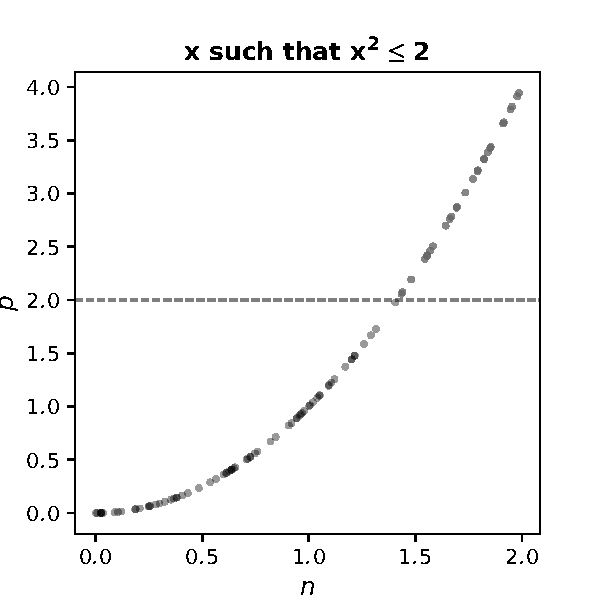
\includegraphics[width=0.8\linewidth]{../drawings/p2_2}
	%	\caption{}
	%	\label{fig:path2}
\end{figure}
\end{multicols}


\pagebreak

\section{Generalized Monty Hall}
a)
\begin{lstlisting}
def f(N, max_doors=3, max_cars=1, switch=True):
	max_cars = min(max_cars, max_doors)
	correct = np.zeros(N, dtype=bool)
	doors = np.arange(max_doors)
	
	for i in range(N):
	cars = np.random.choice(doors, size=max_cars, replace=False)
	my_choice = [np.random.randint(0, max_doors)]
	available_doors = np.setdiff1d(doors, np.union1d(cars, my_choice))
	
	host_open = np.random.choice(available_doors, size=1, replace=False)
	
	if switch:
		remaining_doors = np.setdiff1d(doors, host_open )
		remaining_doors = np.setdiff1d(remaining_doors, my_choice)
		my_choice = np.random.choice(remaining_doors, size=1, replace=False)
	
	correct[i] = my_choice in cars
	
	return np.mean(correct)
\end{lstlisting}
\vspace{10pt}
\noindent
$f(\texttt{500000, max\_doors=5, max\_cars=2})\\=0.5333$
\\
\\
\noindent
b)
I am going to count events like Ajarn demoed in class using a table of events as it was more intuitive to me:

\begin{figure}[H]
	\centering
	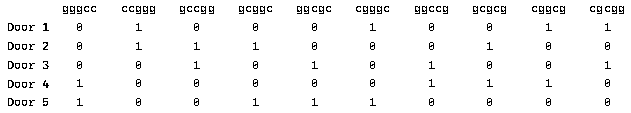
\includegraphics[width=1\linewidth]{../drawings/p3_1}
	%	\caption{}
	%	\label{fig:path2}
\end{figure}

\vspace{-20pt}
\begin{align*}
	P\{\text{Chose C first}\} = \frac{20}{50} = \frac{2}{5} \text{\hspace{10pt}}
	P\{\text{Chose G first}\} = \frac{30}{50} = \frac{3}{5} 
\end{align*}

\vspace{15pt}
\begin{multicols}{2}
\begin{figure}[H]
	\centering
	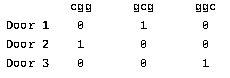
\includegraphics[width=0.75\linewidth]{../drawings/p3_2}
	%	\caption{}
	%	\label{fig:path2}
\end{figure}
\vspace{-25pt}
\begin{align*}
P\{\text{Winning | Chose C First}\} = \frac{3}{9} = \frac{1}{3}\\
\end{align*}



\columnbreak
\begin{figure}[H]
	\centering
	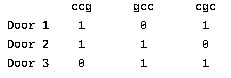
\includegraphics[width=0.75\linewidth]{../drawings/p3_3}
	%	\caption{}
	%	\label{fig:path2}
\end{figure}
\vspace{-25pt}
\begin{align*}
P\{\text{Winning | Chose G First}\} = \frac{6}{9} = \frac{2}{3} \\
\end{align*}

\end{multicols}

\begin{align*}
	P\{\text{Winning}\} = \frac{2}{5}  \cdot \frac{1}{3} + \frac{3}{5}  \cdot \frac{2}{3} = 0.5333...\\
\end{align*}

\section{Truncated Arctan Series From Class}
I did not do TT

\section{Yet another way to approximate π}
Inside \texttt{source/p5.ipynb}

\section{Newton’s Method}
Inside \texttt{source/p6.ipynb}

\section*{Source Code}
\href{https://github.com/AustinMaddison/discrete-simulation/tree/main/hw2/source}{https://github.com/AustinMaddison/discrete-simulation/tree/main/hw2/source}

% References
%\bibliographystyle{unsrt}
%\bibliography{references}

\end{document}
